\chapter{Analýza}\label{chapter:analyza}
% Hlavním cílem této bakalářské práce je implementovat návrh backendu podle návrhu a fragmentu implementace, které byly udělány v rámci předmětů BI-SP1 a BI-SP2 bakalářského studia vyučovaných na FIT ČVUT v akademickém roce 2018/2019 a 2019/2020. 

%TODO move commit footnote to reserse and git footnote
Tato kapitola se zabývá analýzou již existujícího návrhu a dosavadního stavu implementace. Pro zajištění verze aplikace, která bude předmětem analýzy této kapitoly, uvádím datum ukončení práce na projektu v~rámci předmětu Softwarový týmový projekt 2 (BI-SP2) -- 25. února 2020. Také pro možnost pohodlného vyhledání konkrétní verze  (\url{https://gitlab.fit.cvut.cz/rozvody/be-springboot}), uvádím poslední \texttt{commit} provedený přes distribuovaný systém řízení verzí -- Git -- v~rámci tohoto předmětu: 
\begin{quote}
    \enquote{252b0288dbfe9942446b78fd452c0edce810a370}
\end{quote}

\section{Předmět Softwarový týmový projekt 1}\label{analyza:navrh:sp1}
    % TODO REST footmote to first mention
    V~rámci předmětu Softwarový týmový projekt 1 (BI-SP1) pracovalo sedm lidí včetně autora této práce. Tým měl za úkol analyzovat požadavky zákazníka a navrhnout implementaci aplikace. Během semestru tým provedl kompletní analýzu požadavků zákazníka. Tým navrhl scénáře užití aplikace:
    \begin{itemize}
	   \item Přihlašování/Registrace;
	   \item Přihlašování/Registrace do rodiny;
	   \item Role v~aplikaci a jejich vytváření;
	   \item Nastavení pečovatelských dnů;
	   \item Kalendář;
	   \item Kniha potřeb dítěte;
	   \item Uchování účtenek;
	   \item Správa alimentů.
	\end{itemize}
    Potom byl navržen diagram užití\footnote{Popisuje chování systému z~vnějšího pohledu.} a diagram aktivit\footnote{Zobrazuje jak objekty spolupracují.}, podle kterých byl navrženy drátový model pro frontendovou část aplikace a doménový model\footnote{Náčrt základních entit systému a vztahů mezi nimi.} pro backendovou část aplikace. 
    
    Výsledný návrh aplikace se skládá ze dvou částí. Frontendová část aplikace je reprezentována Android aplikací, kterou současně řeší kolega Martin Beran v~rámci své bakalářské práce. Backendová část aplikace, která je předmětem této bakalářské práce, je reprezentována serverovým backendem poskytující REST API pro Android aplikaci.

    % Serverového backendu, který je předmětem této bakalářské práci a frontendové částí aplikace, kterou současně řeší kolega -- Martin Beran -- v rámci bakalářské prací. Frontendová část aplikace je Android aplikací. Backendová část je serverovým backendem, poskytujícím REST\footnote{Representational State Transfer} API pro Android aplikaci.

\section{Předmět Softwarový týmový projekt 2}\label{analyza:navrh:sp2}
    %TODO gradle footnote to reserse and Spring footnote
    Cílem předmětu Softwarový týmový projekt 2 (BI-SP2) byla implementace návrhu předmětu BI-SP1. Autor této práce pracoval v~backendovém týmu a zároveň vystupoval v~roli vedoucího backendového týmu.
    
    Pro vývoj backendove části aplikace byl zvolen jazyk Kotlin, zmíněný v~sekci \ref{resere:kotlin}, a framework Spring, zmíněný v~sekci \ref{resere:j2ee}. Jako nástroj pro automatizaci sestavování programu byl zvolen nástroj Gradle. Podrobněji  budou výsledky předmětu BI-SP2 probrány v~sekci \ref{analyza:soucasnaImplementace}.
        
    
\section{Doménový model}\label{analyza:navrh:DomainModel}
    Hlavním zdrojem informace o~výsledném návrhu serveru je doménový model. Kompletní doménový model se nachází v~příloze \ref{dodatek:DomainModel}. Během implementace tým označoval entity, které jsou kompletně nebo částečně implementovány. Zelenou barvou jsou označeny třídy, které už jsou implementovány. Žlutou barvou jsou označeny třídy, které ještě nejsou implementovány. Třídy označené zároveň žlutě i zeleně jsou implementovány pouze částečně. Tento doménový model má nedostatky detekované při implementaci, jak frontendové, tak i backendové části aplikace. Jako příklad takových nedostatků je možné uvést zbytečně komplikovaný návrh entity \texttt{Interval} (viz obrázek \ref{image:Interval1}). Podrobný popis tohoto problému bude uveden v~sekci \ref{analyza:pozadavky-frontendu}.

\section{Analýza předešlého návrhu} \label{analyza:analyza navrhu}
    V~této sekci budou podrobně popsány klíčové aspekty aplikace podle již existujícího návrhu aplikace. Problémy a navržené změny těchto části budou popsány v~následujících sekcích.

    \subsection{Registrace a přihlášeni do systému}
        Aplikace je navržena takovým způsobem, že první uživatel, který má vytvořit svůj účet je jeden z~rodičů. Pro registraci je potřeba řada povinných údajů:
        \begin{itemize}
	        \item jméno -- zvolené jméno se stává implicitním jménem v~systému;
	        \item příjmení -- zvolené příjmení se stává implicitním příjmením v~systému;
	        \item e-mailová adresa -- zvolený e-mail je identifikátorem uživatele v~rámci systému;
	        \item heslo -- heslo pro autorizaci v~systému.
        \end{itemize}
        Na základě těchto údajů se vytvoří unikátní uživatel v~rámci systému. V~tento okamžik uživatel není přihlášen do žádné rodiny a nemá žádnou roli. Podrobněji budou role popsané v~sekci \ref{analyza:bezpecnost:role}.
        % \begin{figure}\centering
	       % 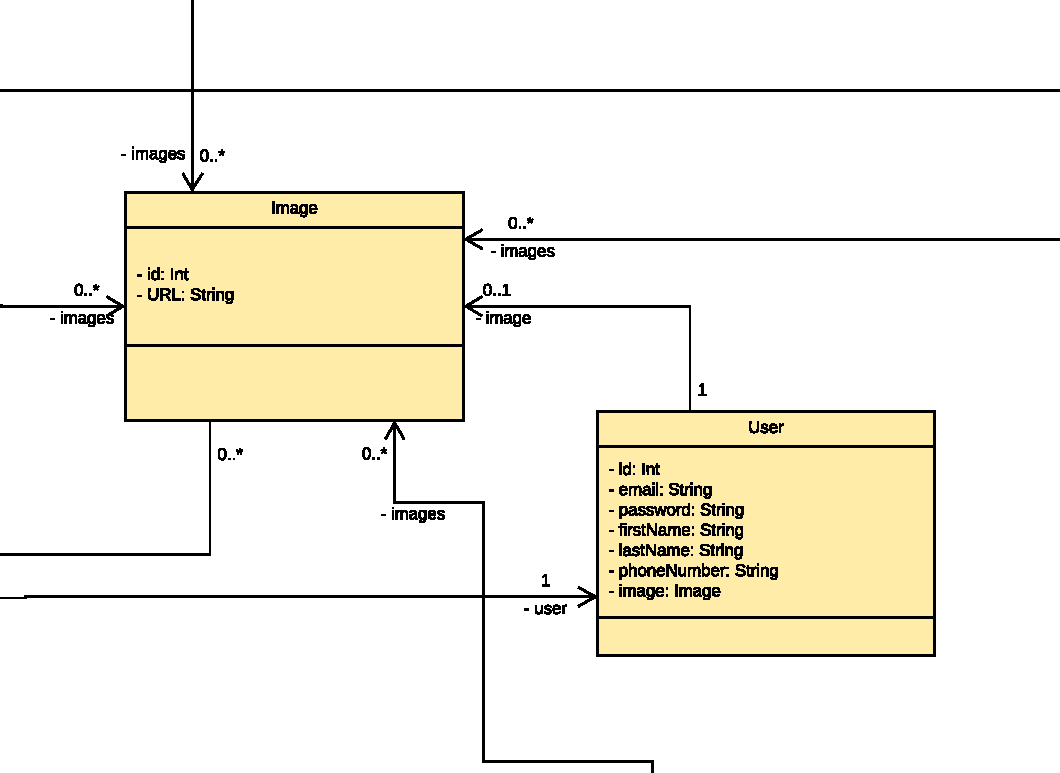
\includegraphics[width=0.7\textwidth]{pdfs/User-Image1}
	       % \caption[Návrh User-Image]{Vztah mezi třídami \texttt{User} a \texttt{Image} podle Doménového modelu z předmětu BI-SP2}\label{image:User-Image1}
        % \end{figure}
        
        Potom má uživatel možnost vytvořit rodinu nebo se přihlásit do již existující rodiny. Pro vytvoření nové rodiny, potřebuje uživatel zadat jméno rodiny a přidat členy rodiny. Autor této rodiny se automaticky stává jedním z~rodičů této rodiny. Jinou možností je se přihlásit do rodiny, která již existuje. Podmínkou je pozvání do některé existující rodiny, což znamená, že přidat nového uživatele do rodiny může jenom člen této rodiny. V~takovém případě uživatel už nemá možnost zvolit role v~rámci rodiny. Role má být nastavena uživatelem, který vytvořil toto pozvání.

    \subsection{Kalendář}    
        Kalendář je nejdůležitějším zdrojem informaci pro celou rodinu a je společný pro~všechny uživatele. Na něm jsou zobrazené pečovatelské dny obou rodičů zvýrazněné různými barvami. Kalendář též zobrazuje jednorázové a pravidelné události.
        
        \begin{figure}\centering
	        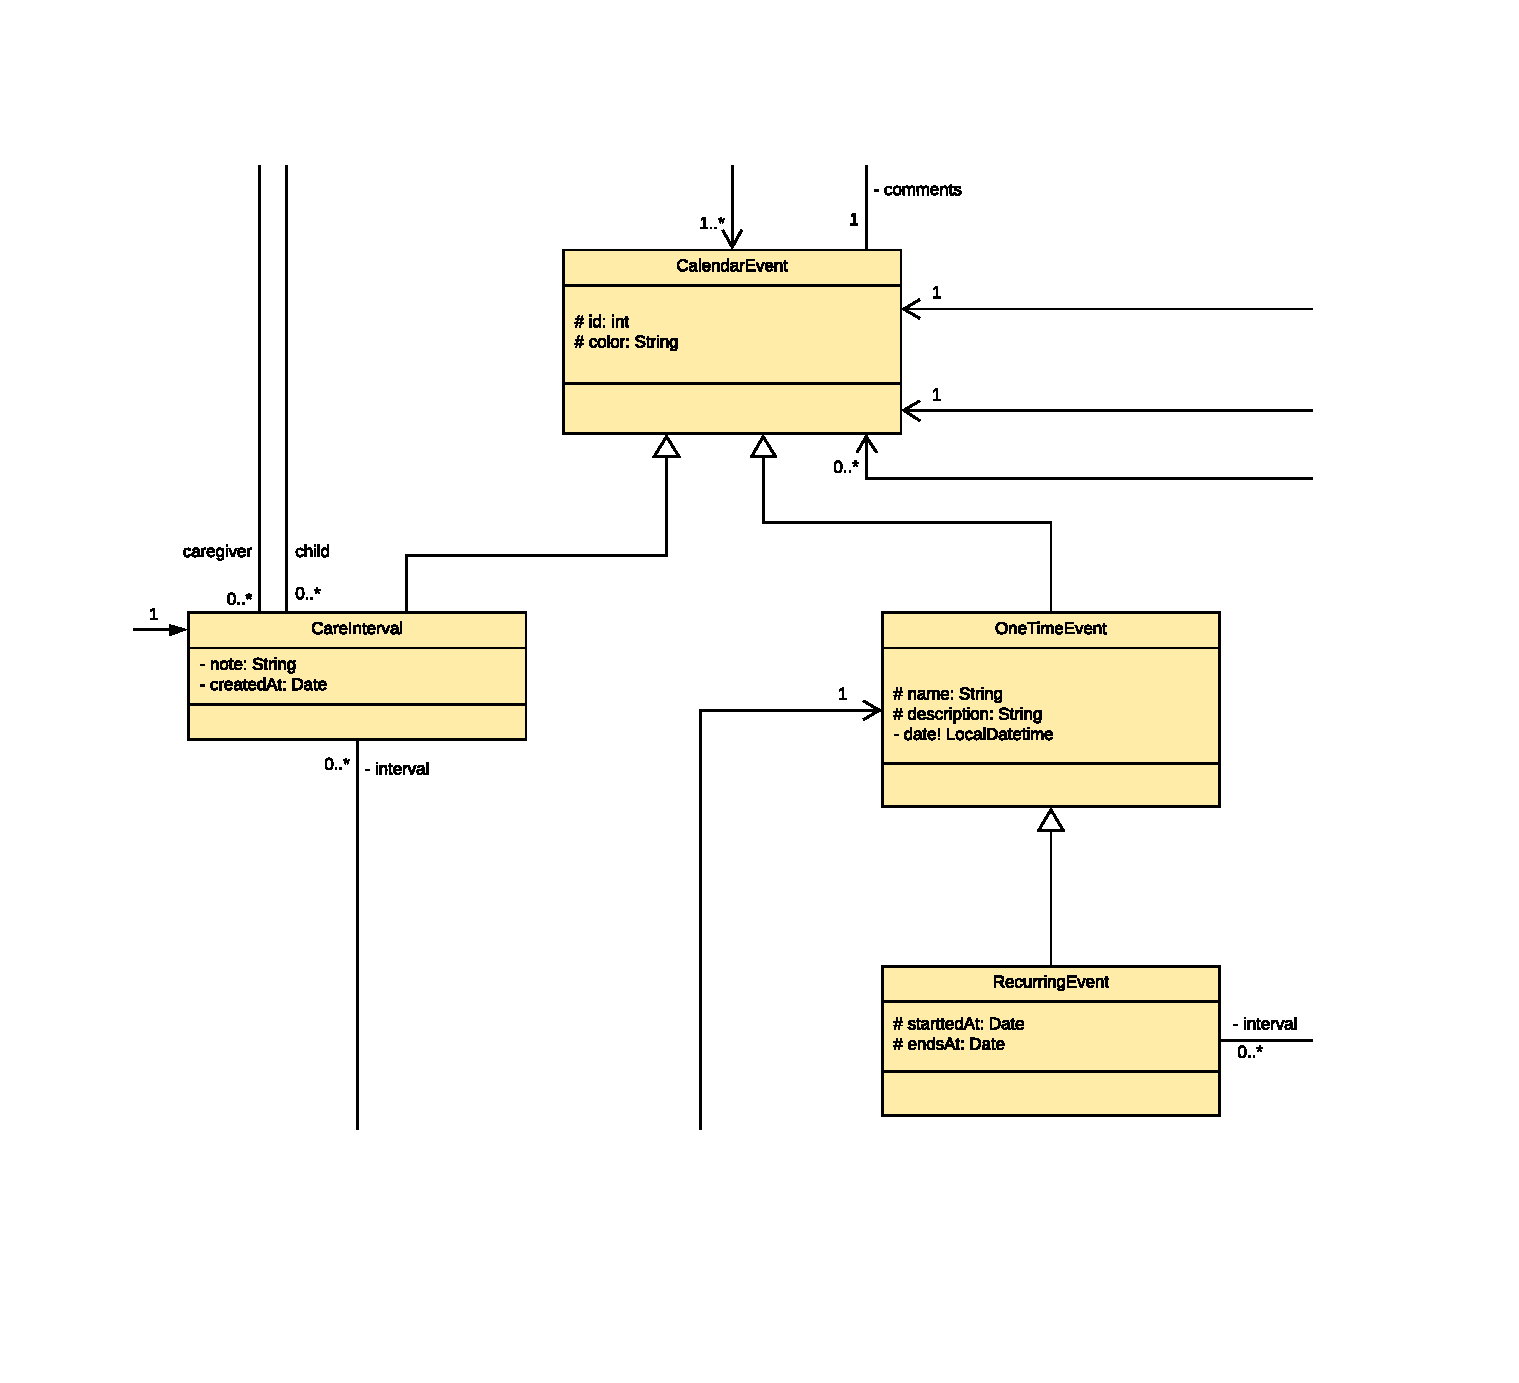
\includegraphics[width=1.0\textwidth]{pdfs/CalendarInfo1}
	        \caption[Předešlý návrh kalendáře]{Návrh kalendáře podle doménového modelu z~předmětu BI-SP2}\label{image:calendar-info}
        \end{figure}
        Doménový model neobsahuje informace o~kalendáři, ale obsahuje entity reprezentující informaci, kterou kalendář bude zobrazovat (viz obrázek \ref{image:calendar-info}). Každý element, který bude zobrazen v~kalendáři, je reprezentován stejnou entitou \verb|CalendarEvent|. Entita obsahuje jenom informaci o~barvě, kterou událost bude zobrazená v~kalendáři a závislost na entitě \verb|Comment|. Za reprezentaci pečovatelských dnů odpovídá entita \verb|CareInterval|, která se dědí od entity \verb|CalendarEvent|. Za reprezentaci jednorázových a opakujících se~událostí odpovídají entity \verb|OneTimeEvent| a \verb|RecurringEvent|, kde se \verb|RecurringEvent| dědí od \verb|OneTimeEvent|.
        
        % Současný návrh kalendáře nepokrývá všechny scénáře použití. Podrobný popis problémů a navržené změny budou uvedeny v sekci \ref{analyza:kalendar}. 
        
        % Kromě dlouhodobých nastavení pečovatelských dnu, kalendář může zobrazovat i jednorázové změny, které mohou vidět všechny členy rodiny. 
    \subsection{Alimenty}
        \begin{figure}\centering
	        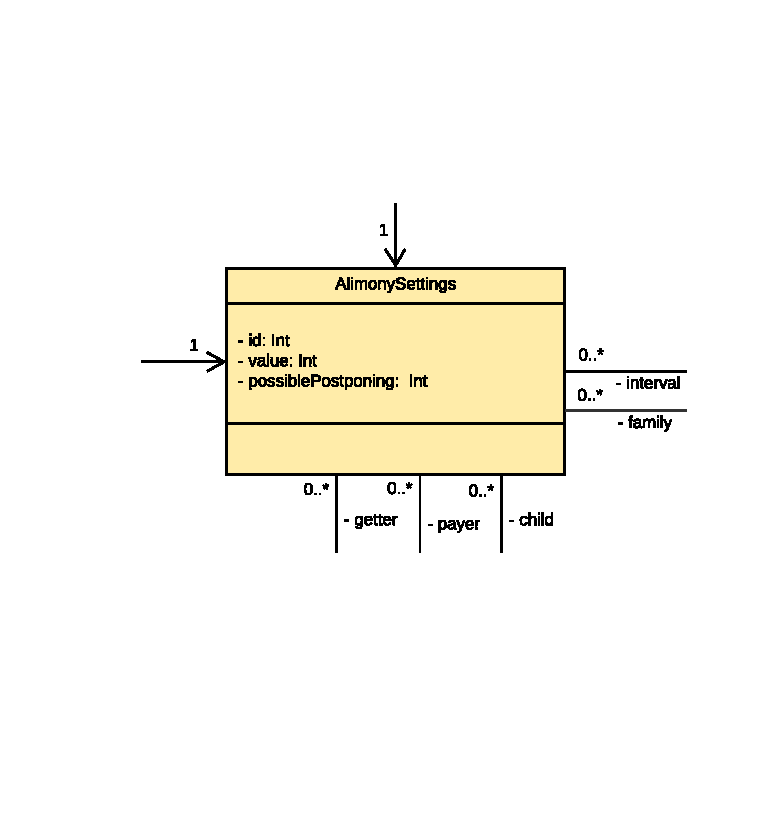
\includegraphics[width=0.7\textwidth]{pdfs/AlimonySettings1}
	        \caption[Návrh entity \texttt{AlimonySettings}]{Návrh entity \texttt{AlimonySettings} podle doménového modelu z~předmětu BI-SP2}\label{image:AlimonySettings1}
        \end{figure}
        \begin{figure}\centering
	        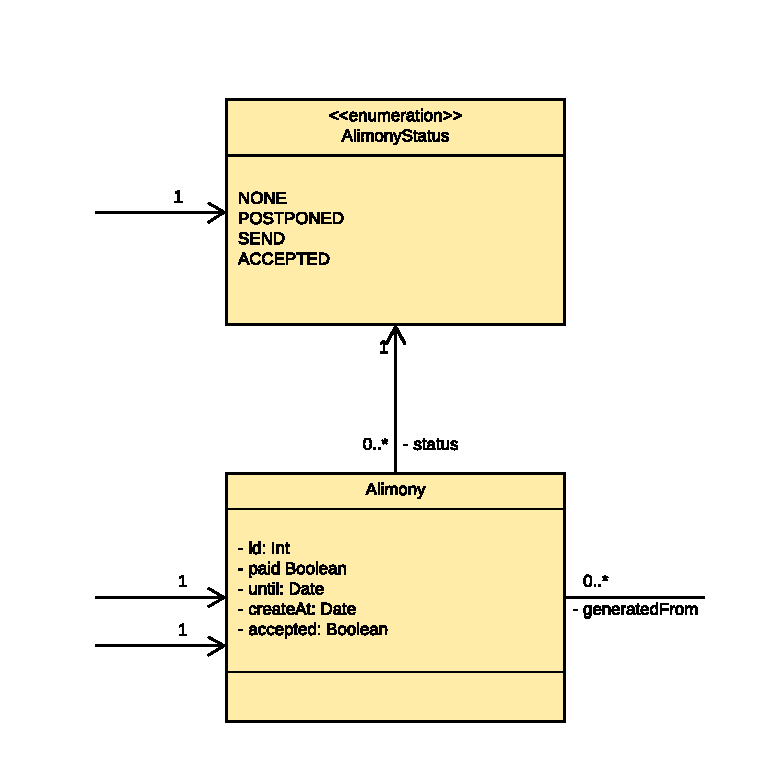
\includegraphics[width=0.8\textwidth]{pdfs/Alimony1}
	        \caption[Návrh entity \texttt{Alimony}]{Návrh entity \texttt{Alimony} podle doménového modelu z~předmětu BI-SP2}\label{image:Alimony1}
        \end{figure}
        Důležitou částí aplikace je správa alimentů, které má pravidelně uhrazovat jeden z~rodičů. Tento proces byl rozdělen do dvou částí. První částí je dlouhodobé nastavení alimentů (viz obrázek \ref{image:AlimonySettings1}). Druhou částí jsou samotné alimenty (viz obrázek \ref{image:Alimony1}), které se generují na základě dlouhodobých nastavení. Jedna rodina může mít zároveň několik nastavení v~případě, že rodina má několik dětí nebo chce rozdělit alimenty do logických bloků.
        
        Každá instance alimentů má stav, který se postupně mění. V~moment vytvoření instance má stav \verb|NONE|. Po odeslání alimentů druhému rodiči se stav mění na \verb|SEND|. Druhý rodič následně potvrdí, že alimenty přijal a tím se změní stav stav na \verb|ACCEPTED|. Také může nastat situace, kdy rodič nemá možnost odeslat alimenty včas. V~takovém případě se stav instance mění na \verb|POSTPONED|.
    
    \subsection{Kniha potřeb dítěte}\label{analyza:navrh:need}
        \begin{figure}\centering
	        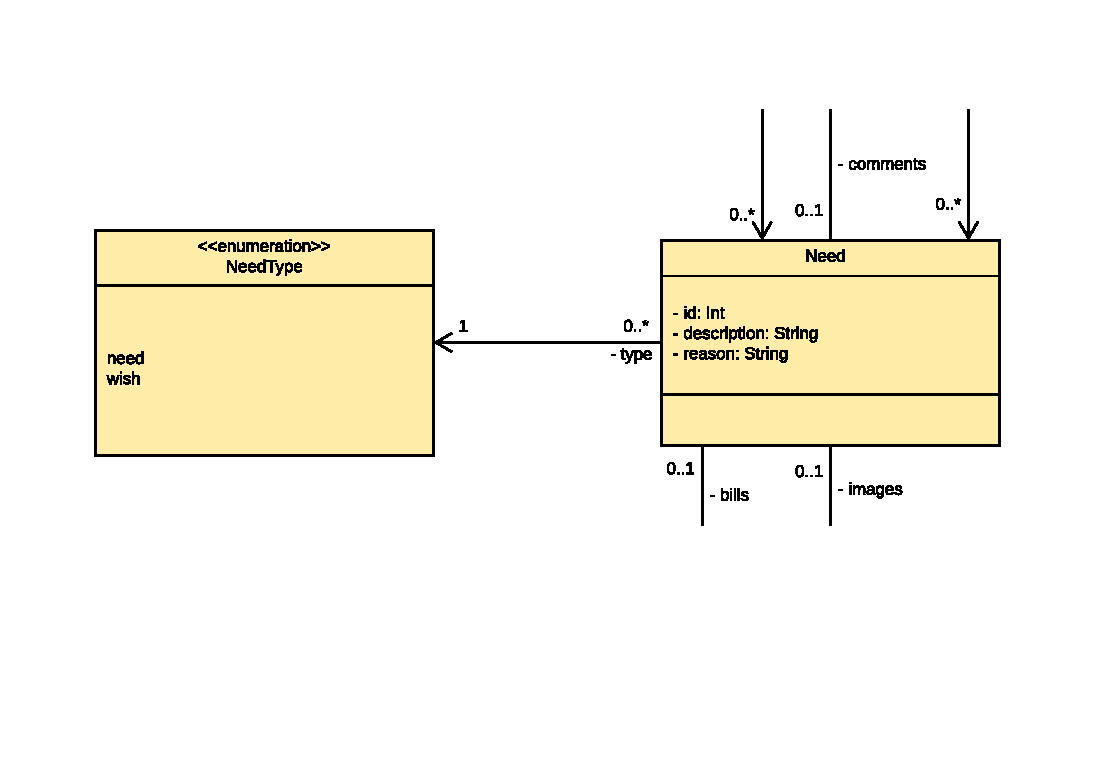
\includegraphics[width=1.0\textwidth]{pdfs/Need1}
	        \caption[Návrh \texttt{Need}]{Návrh entity \texttt{Need} podle doménového modelu z~předmětu BI-SP2}\label{image:Need1}
        \end{figure}
        Jedním s~častých problémů, které vznikají během procesu rozvodu, je nakupování příliš drahých dárků, o~kterých ostatní členové rodiny nevědí. Jako příklad je možné uvést nakupování bot pro dítě. Jeden z~rodičů si může chtít \enquote{koupit lásku dítěte} a koupí několikanásobně dražší boty než, dítě ve skutečnosti potřebuje. Kniha potřeb dítěte (viz obrázek \ref{image:Need1}) je zaměřena na překonání takových situací.
        
        % \begin{figure}\centering
	       % 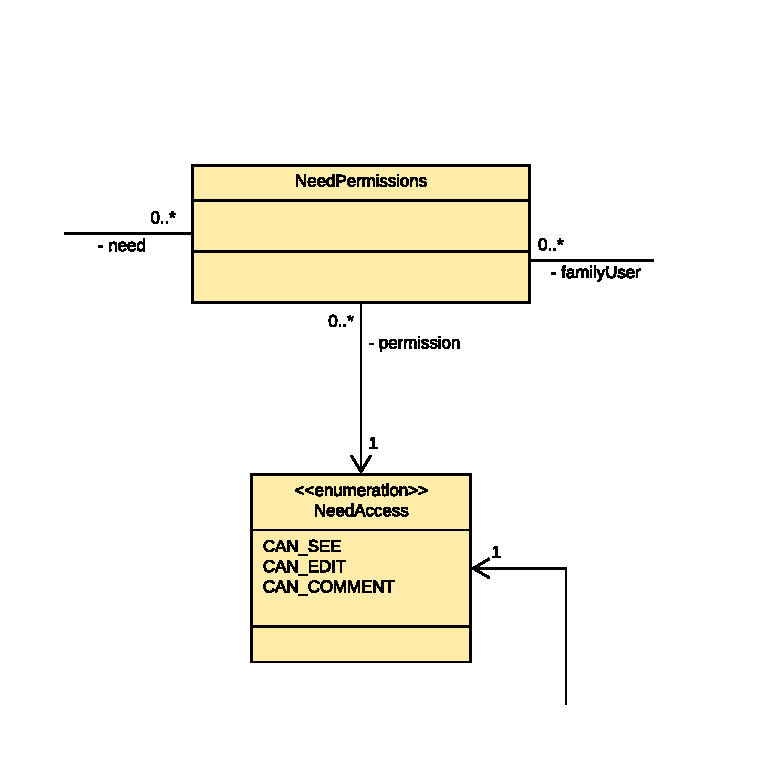
\includegraphics[width=0.8\textwidth]{pdfs/NeedPermissions1}
	       % \caption[Návrh entity \texttt{NeedPermissions}]{Návrh entity \texttt{NeedPermissions} podle doménového modelu z~předmětu BI-SP2}\label{image:NeedPermissions1}
        % \end{figure}
        Potřeba může být typu \verb|need| nebo \verb|wish|. Podle dosavadního návrhu je rozdíl mezi typy pouze pro informační účely. Každé instanci entity \verb|Need| patří instance entity \verb|NeedPermission| (viz obrázek \ref{image:NeedPermissions1}), která definuje přístupová práva pro jednotlivé členy rodiny. V~případě, že uživatel nemá žádné z~přístupových práv, potřeba se nevyskytuje v~jeho seznamu potřeb dítěte. Toto~pravidlo se netýká jenom rodičů, kteří mají přístup ke všem potřebám automaticky.
       
       Potřeba obsahuje následující informaci:
        \begin{itemize}
            \item popis -- popis potřeby;
            \item příčina -- příčina, proč dítě toto potřebuje;
            \item obrázky -- obrázky věcí, které dítě potřebuje;
            \item účtenky -- účtenky v~případě, že někdo z~rodičů splnil potřebu;
            \item komentáře -- komentáře členu rodiny včetně dítěte.
        \end{itemize}
    
    \subsection{Účtenky}
        \begin{figure}\centering
	        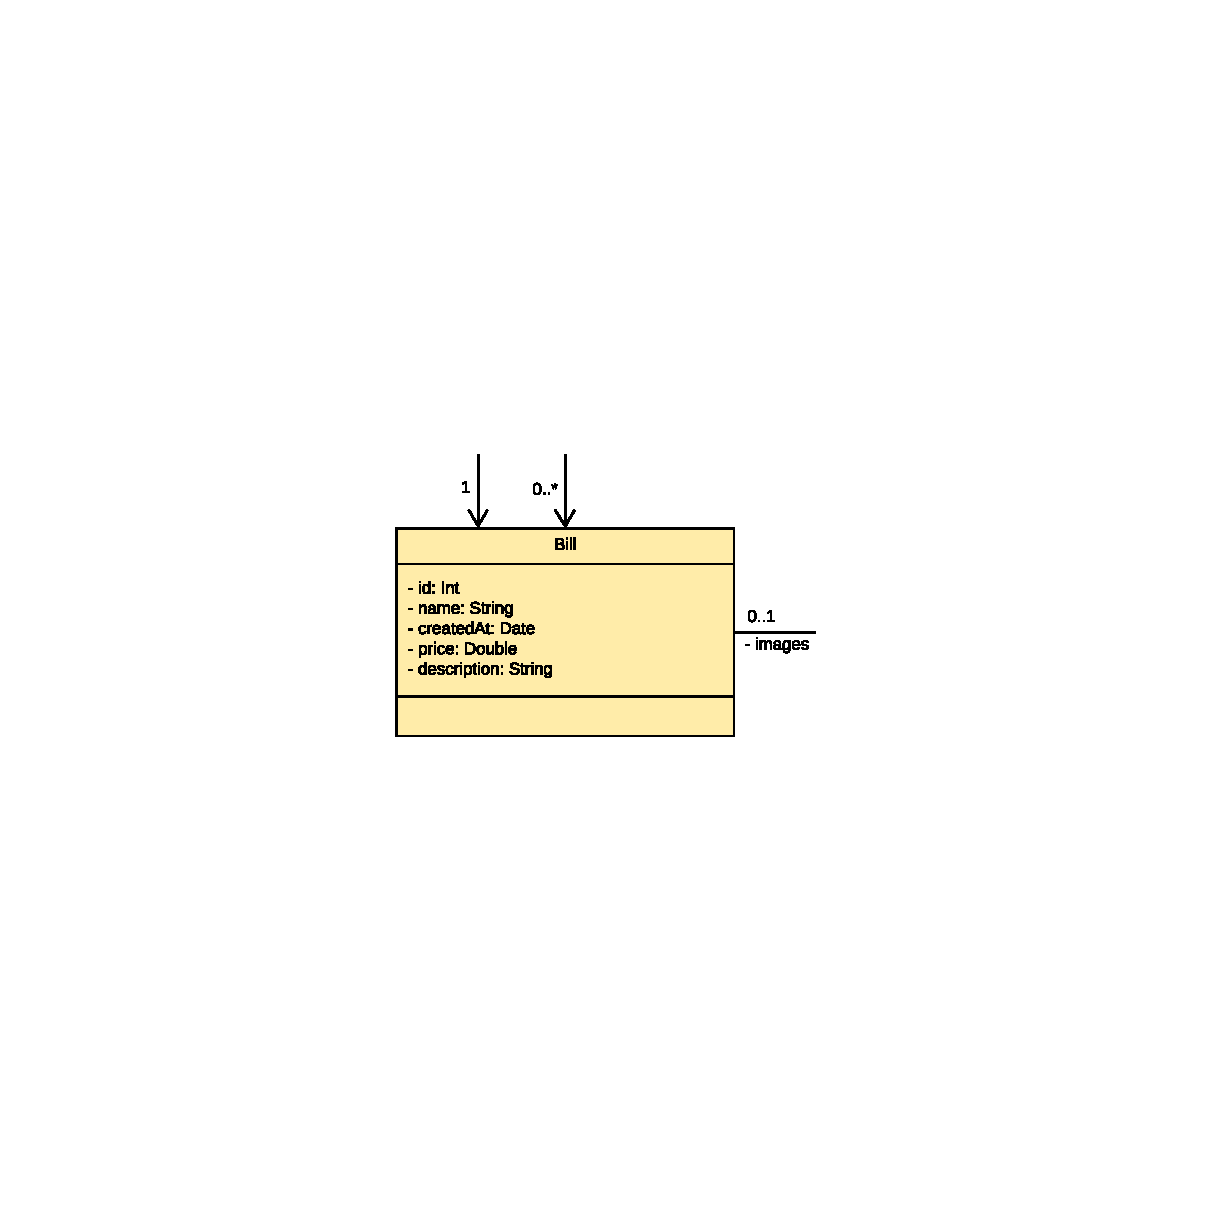
\includegraphics[width=0.6\textwidth]{pdfs/Bill1}
	        \caption[Návrh entity \texttt{Bill}]{Návrh entity \texttt{Bill} podle doménového modelu z~předmětu BI-SP2}\label{image:bill1}
        \end{figure}
        V~sekci \ref{analyza:navrh:need} už bylo zmíněno, že je potřeba řešit problém nakupování dárků pro dítě, ale kniha potřeb dítěte řeší tento problém jenom částečně. Nikdo nezabrání uživateli uvést v~popisu splněného požadavku nebo potřeby neplatné údaje, proto byla zavedena možnost přidání účtenky (viz obrázek \ref{image:bill1}). Tato entita, kromě údajů o~nakoupeném zboží, umožňuje přidání fotografií potvrzujících platnost uvedených údajů.
    
    \subsection{Požadavky na změny}
        Každý člen rodiny může udělat určité změny v~rámci rodiny. Například nastavit přezdívku pro konkrétního uživatele nebo přidat fotografii do události v~kalendáři. Každá taková změna je důležitá, ale jsou změny, které by měly být kontrolovány rodiči. Pro zaručení kontroly byly zavedeny požadavky na~změny pro některé změny v~rámci rodiny. Následně, pro provedení změny v~příslušných entitách uživatel potřebuje nejdřív vytvořit požadavek a schválit ho.
        Právo na schválení nebo zamítnutí požadavků mají jenom rodiče. Požadavky, které byly vytvořeny jedním z~rodičů, mají být potvrzeny druhým rodičem. Ostatní požadavky musí být potvrzeny oběma rodiči. Seznám požadavků se~skládá z:
        \begin{itemize}
            \item \texttt{AlimonySettingRequest} -- požadavek na změnu nastavení alimentů, který může být vytvořen jedním z~rodičů;
            \item \texttt{AlimonyChangeRequest} -- požadavek na změnu stavu instance alimentů, který může být vytvořen jedním z~rodiců;
            \item \texttt{OneTimeEventRequest} -- požadavek na vytvoření jednorázové události v~kalendáři, který může být vytvořen jakýmkoliv členem rodiny;
            \item \texttt{OneTimeEventChangeRequest} -- požadavek na změnu již existující události v~kalendáři, který může být vytvořen jakýmkoliv členem rodiny;
            \item \texttt{ChildItemRequest} -- požadavek na změnu nastavení pečovatelských dnů, který může být vytvořen jakýmkoliv členem rodiny. Změna může být jak jednorázová, tak i dlouhodobá.
        \end{itemize}
        \begin{figure}\centering
	        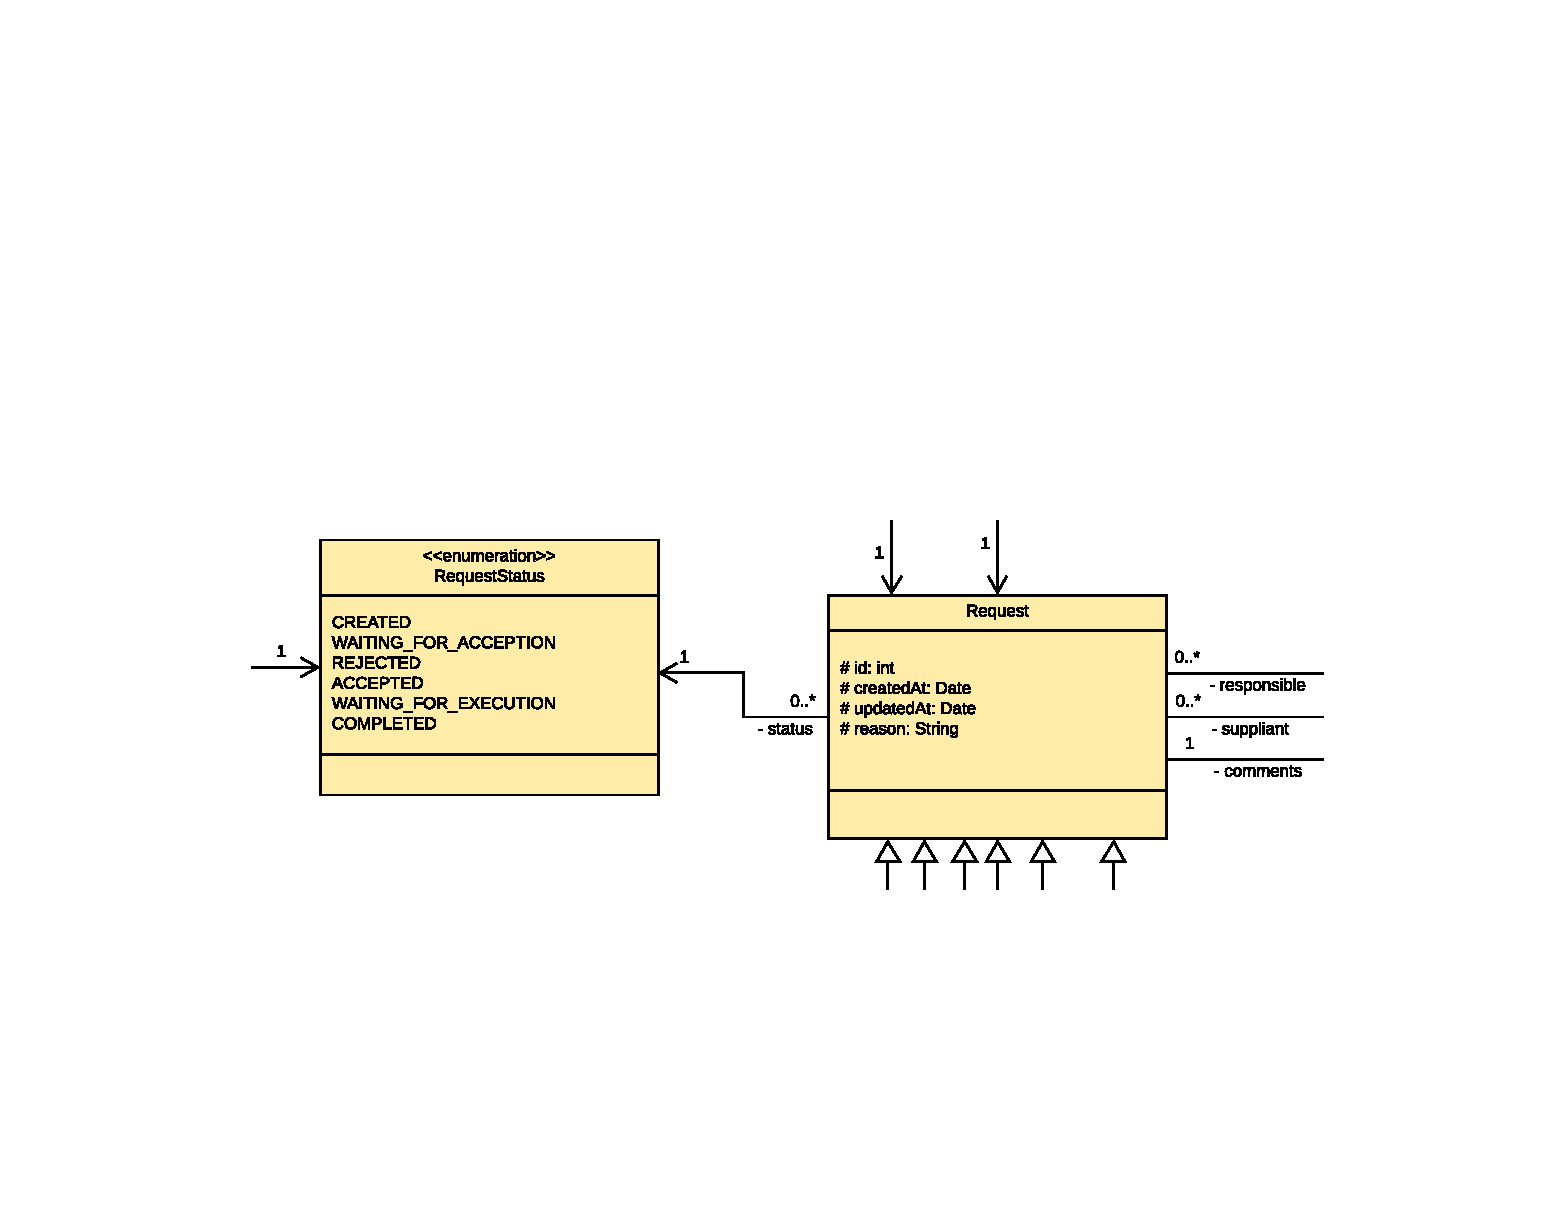
\includegraphics[width=1.0\textwidth]{pdfs/Abstr-Requrest1}
	        \caption[Návrh abstraktní entity \texttt{Request}]{Návrh abstraktní entity \texttt{Request} podle doménového modelu z~předmětu BI-SP2}\label{image:abstr-request1}
        \end{figure}
        Každá entita požadavku je zděděna od společné abstraktní entity \verb|Request| obsahující základní informace o~požadavku (viz obrázek \ref{image:abstr-request1}). Mezi základní informace patří datum vytvoření, datum poslední změny, příčina a také aktuální stav požadavku. Také tato entita obsahuje závislosti na základních aktérech tohoto požadavku a komentáře.
        
        Stavy požadavků reprezentují jejich životní cyklus. Při vytvoření každý požadavek má stejný stav -- \verb|CREATED|. Po potvrzení požadavku jeho autorem má požadavek stav \verb|WAITING_FOR_ACCEPTING|. Po schválení rodiči se stav mění na~\verb|ACCEPTED| nebo na \verb|WAITING_FOR_EXECUTION| v~případě, že je změna akceptována, ale~ještě není uplatněna. Též může nastat případ, že byl požadavek zamítnut, pak se stav mění na \verb|REJECTED|. Požadavek je zamítnut v případě, že alespoň jeden z rodičů ho zamítl. V~okamžik, kdy je požadavek schválen nebo se čeká na uplatnění, není možné měnit položky tohoto záznamu.
    
    \subsection{Historie změn}
        Každá provedená v rámci rodiny změna má význam při debatách mezi rodiči. Podle požadavků zákazníka by všechny změny v~rámci rodiny měly být zaznamenány. Proto byly zavedeny entity historií, které kopírují všechny položky entit a přidávají datum vytvoření záznamu a odkaz do patřičné entity v~případě, že tato příslušná entita byla aktualizována. Takové entity jsou zavedeny jenom pro důležité části aplikace, které mohou být změněny uživatelem:
        \begin{itemize}
            \item \texttt{CalendarEventHistory};
            \item \texttt{BillHistory};
            \item \texttt{AlimonyHistory};
            \item \texttt{AlimonySettingsHistory};
            \item \texttt{RequestHistory}.
        \end{itemize}
        Všechny typy historie jsou zděděny od stejné entity -- \verb|History|. Tato entita obsahuje základní údaje pro libovolný typ historie: ID\footnote{identifikátor} a datum vytvoření záznamu. 
     
\section{Analýza předešlé implementace}\label{analyza:soucasnaImplementace}
    \begin{figure}\centering
	   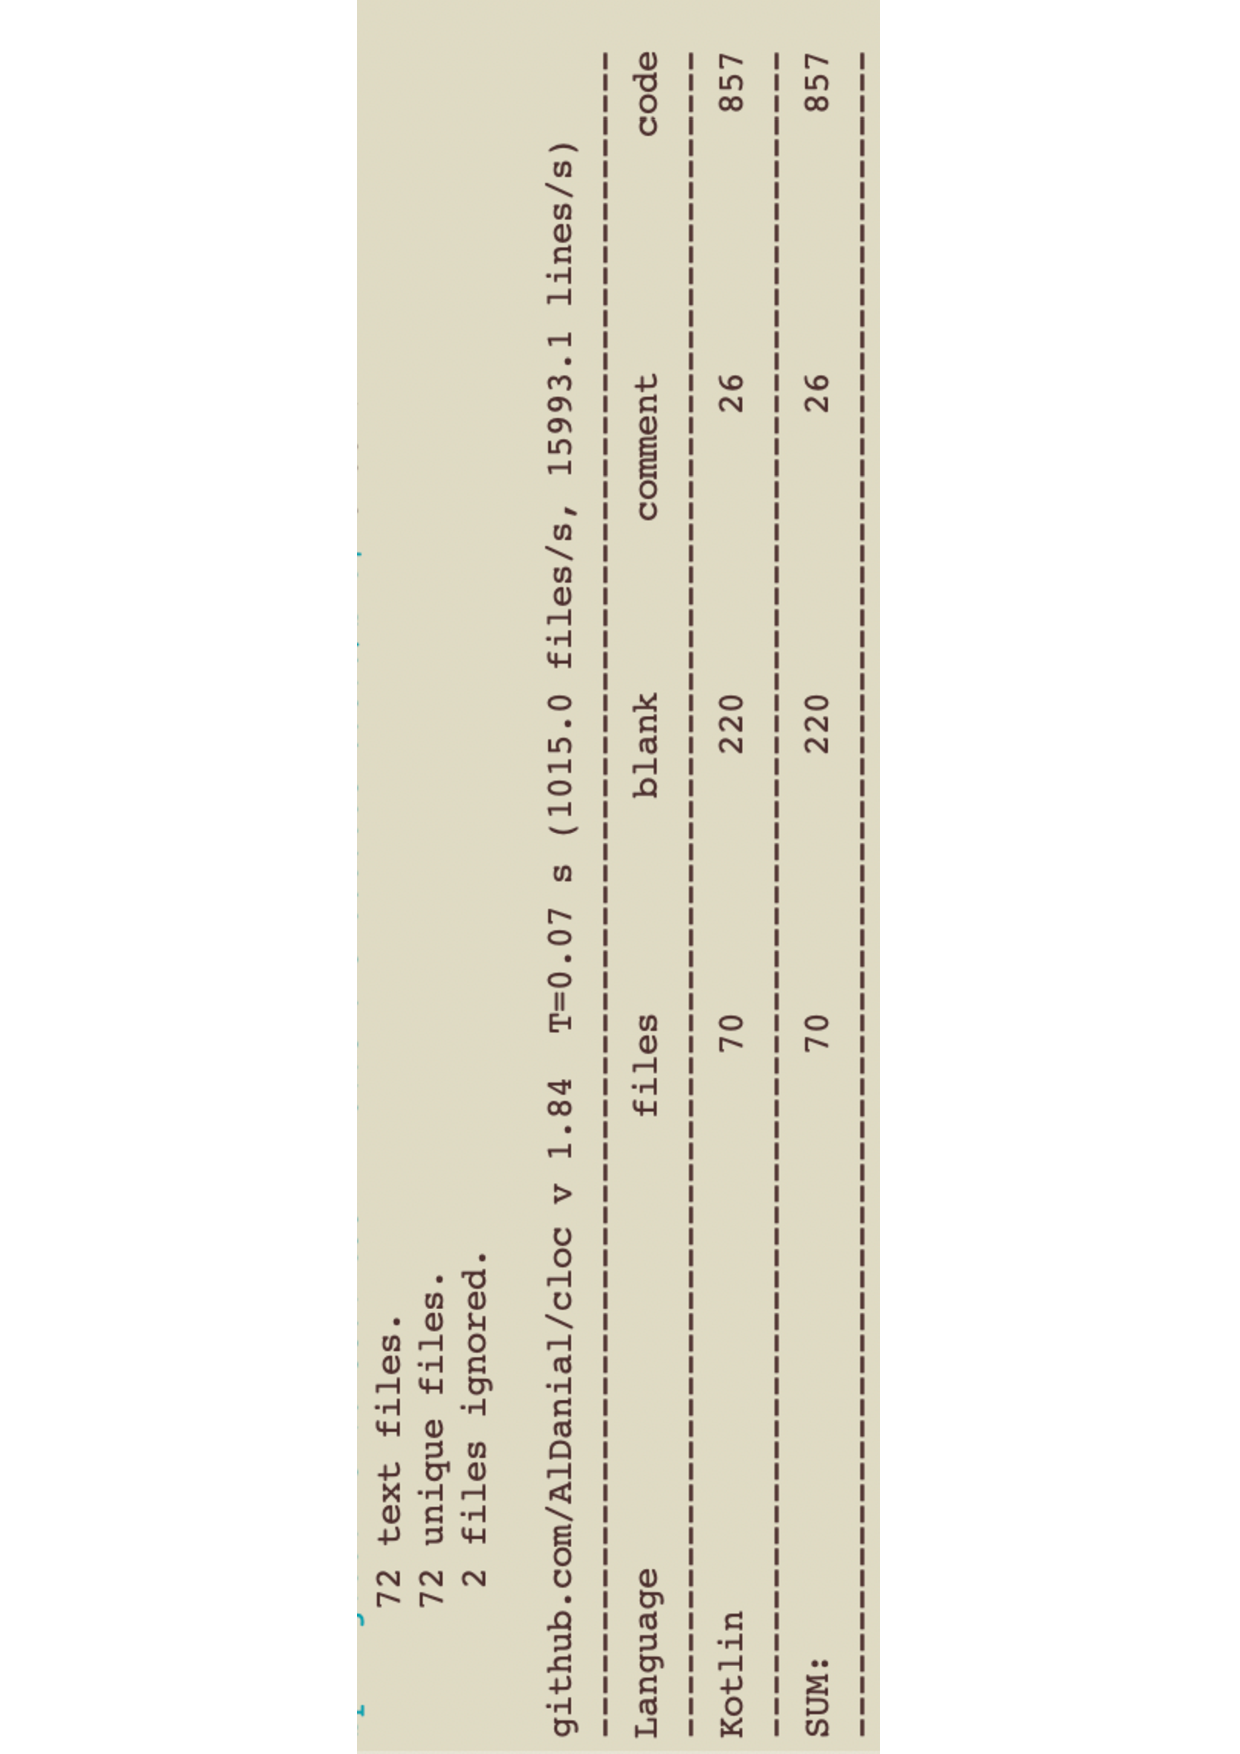
\includegraphics[angle=-90, width=0.9\textwidth]{pdfs/Cloc1}
	   \caption[Počet řádků kódu před začátkem práce]{Počet řádků kódu před začátkem práce}\label{image:cloc1}
    \end{figure}
    Dosavadní implementace obsahuje 69 souborů a 845 řádek kódů (viz~obrázek~\ref{image:cloc1}). Práce byla provedena členy týmu předmětu BI-SP2. Za účelem zpřesnění analýzy byl zvolen nástroj pro analýzu počtu řádek kódu, který byl popsán v~sekci \ref{reserse:cloc}. Implementace částečně pokrývá doménový model zmíněný v~sekci \ref{analyza:navrh:DomainModel}. V~této sekci budou popsány již implementované části aplikace. 
     
    Pro implementaci serverového backendu byla zvolena architektura REST skládající se ze tří vrstev:
    \begin{itemize}
         \item Aplikační vrstva, která pokrývá scénáře využití aplikace;
         \item Doménová vrstva, která obsahuje logiku aplikace;
         \item Datová vrstva, která komunikuje s~databází.
    \end{itemize}
    
    Pro implementaci datové vrstvy byl použit framework Spring Data, který byl popsán v~sekci \ref{resere:j2ee}. Nástroj přidává dodatečnou vrstvu pro implementaci JPA a tím zrychluje a zjednodušuje implementaci. Pro implementaci této vrstvy bylo zvoleno rozhraní \verb|CrudRepository|, které vyžaduje uvedení typu doménové třídy a typu identifikátoru. Každé entitě patří jedna taková třída pro~práci s~databází.
    
    Pro implementaci doménové vrstvy byly pro každou entitu přidány rozhraní reprezentující funkci, které je možné provádět s~příslušnou entitou. Implementace byla oddělená od definicí metod pro zvětšení modularity výsledného softwaru. Implementace této vrstvy přímo komunikuje s~datovou vrstvou. Provázání tříd se vzniká na základě vkládání závislostí. Proces vkládaní řídí framework Spring podle principu IoC. Tato vrstva komunikuje s~datovou vrstvou pomocí reprezentací entit, ale s~aplikační vrstvou komunikuje pomocí Data Tranfer Object (DTO). Konverzace z~entity na DTO se provádí v~příslušné třídě entity. Konverzace z~DTO na entitu se provádí v~příslušné třídě DTO.
    
    % http requests https://www.ibm.com/support/knowledgecenter/SSGMCP_5.2.0/com.ibm.cics.ts.internet.doc/topics/dfhtl21.html
    Aplikační vrstva je reprezentována sadou řadičů (\textit{controllers}), kde každý řadič je určen pro konkrétní aspekt použití aplikace. Pro~každý řadič je vymezená samostatná cesta, která se zadává jako řetězec požadavku \cite{http-request-components}. Tato vrstva přímo komunikuje s~doménovou vrstvou. Provázání tříd se provádí také pomocí vkládaní závislostí. Komunikace aplikační vrstvy přes API se provádí pomocí DTO.
    
    \subsection{Implementované entity}\label{analyza:implementace:tridy}
        Seznam implementovaných entit:
        \begin{itemize}
            \item \texttt{AlimonyStatus};
            \item \texttt{Bill};
            \item \texttt{CalendarEvent};
            \item \texttt{OneTimeEvent};
            \item \texttt{Comment};
            \item \texttt{FamilyMember} -- je přítomná pouze část implementace;
            \item \texttt{History};
            \item \texttt{IntervalType};
            \item \texttt{NWeekInterval};
            \item \texttt{WeekInterval};
            \item \texttt{NeedAccess};
            \item \texttt{NeedType};
            \item \texttt{AbstractPermissions};
            \item \texttt{Permissions};
            \item \texttt{RequestStatus};
            \item \texttt{User}.
        \end{itemize}
        
        \begin{table}[h]\centering
	    \begin{tabular}{|l|c|c|c|}\hline
		  Typ chyby		& HTTP status		& zpáva	& URL	\tabularnewline \hline \hline
		  \texttt{Illegal Access}	& 401	& původní zpráva chyby		& původní cesta     \tabularnewline \hline
		  \texttt{Illegal Argument}	& 400	& původní zpráva chyby		& původní cesta     \tabularnewline \hline
		  \texttt{Null Pointer}	& 500	& původní zpráva chyby		& původní cesta     \tabularnewline \hline
		  \texttt{No Such Element}	& 404	& nic		& nic     \tabularnewline \hline
	    \end{tabular}\caption[Konfigurace našeptávače pro řadiče]{Ukázka konfigurace našeptávače zachycování výjimek pro řadiče}\label{tab:excpetion-handler1}
        \end{table}
        \begin{figure}[h]\centering
            \begin{minted}
        [frame=lines,
        framesep=2mm,
        baselinestretch=1.2,
        fontsize=\footnotesize,
        linenos]{java}
@Configuration
@EnableSwagger2
class SwaggerConfig {
@Bean
fun api(): Docket {
    return Docket(DocumentationType.SWAGGER_2)
        .select()
        .apis(RequestHandlerSelectors.any())
        .paths(PathSelectors.any())
        .build()
    }
}
            \end{minted}
            \caption{Ukázka nastavení frameworku Swagger}\label{code:swagger-configuration}
        \end{figure}
        Kromě kostry aplikace, která zaručuje třívrstvou architekturu, byly také implementovány pomocné třídy zlepšující výsledný návrh aplikace. Jednou z~takových tříd je třída, která uvádí nápovědy pro všechny řadiče ohledně zachycování výjimek. Tato třída byla zavedena za účelem poskytnutí uživateli pouze korektně formátované informace a filtrování zbytečných informací pro~koncového uživatele. Konfigurace našeptávače je uvedena v~tabulce \ref{tab:excpetion-handler1}. Jinou pomocnou třídou je řadič určený pro ověření, zda server funguje. Tento řadič je namapován na cestu \enquote{/}.
        
        % Byl přidán \texttt{controller}\footnote{vrstva controlleru zajišťuje REST API komunikaci, překládá výjimky na HTTP kóda zajišťuje omezení pro jednotlivých uživatelů} pro testování, zda aplikace běží, který je namapován\footnote{přidání konkrétnímu controlleru adresy pomocí anotací frameworku Spring, která se zadává jako URI při odesílaní požadavků na Server} na cestu \enquote{/}. Také, byla přidaná třída, která obsahuje nápovědy pro ostatní \texttt{controllery} ohledně zachycování chyb. Tato třída byla zavedena za účelem poskytování uživateli jenom korektně formátovanou informaci  a filtrování zbytečné informace pro koncového uživatele (viz tabulku \ref{tab:excpetion-handler1}). 
        
    
    \subsection{Dokumentace API}
%         \begin{figure}
%             \begin{minted}
%         [frame=lines,
%         framesep=2mm,
%         baselinestretch=1.2,
%         fontsize=\footnotesize,
%         linenos]{java}
% @Configuration
% @EnableSwagger2
% class SwaggerConfig {
% @Bean
% fun api(): Docket {
%     return Docket(DocumentationType.SWAGGER_2)
%         .select()
%         .apis(RequestHandlerSelectors.any())
%         .paths(PathSelectors.any())
%         .build()
%     }
% }
%             \end{minted}
%             \caption{Ukázka nastavení frameworku Swagger}\label{code:swagger-configuration}
%         \end{figure}
        
        Pro dokumentaci API byl zvolen framework Swagger, který již byl zmíněn v~sekci~\ref{resere:dokumentace}. V~předešle implementaci je použitá druhá verze tohoto frameworku. Také byla provedena konfigurace pro generování dokumentace při každém spouštění aplikace na základě do kódu přidaných anotací (viz obrázek \ref{code:swagger-configuration}). Po spuštění aplikace je online dokumentace dostupná na cestě \enquote{/swagger-ui.html}.
    
        % Bylo provedeno nastavení frameworku Swagger pro dokumentace API (viz obrázek \ref{code:swagger-configuration}). Podrobněji framework Swagger byl popsán v sekci \ref{resere:dokumentace}. Po spuštění serveru, dokumentace se automaticky generuje a je přístupná ze stejného portu na cestě \enquote{/swagger-ui.html}.

    \subsection{Profily}\label{analyza:soucasnaImplementace:profily}
    %spring profiles: https://docs.spring.io/spring-boot/docs/current/reference/html/spring-boot-features.html#boot-features-profiles
    %applicatioon peoperties: https://docs.spring.io/spring-boot/docs/current/reference/html/spring-boot-features.html#boot-features-external-config-application-property-files
        Framework Spring, použitý v~předešle implementaci, poskytuje možnost rozdělit aplikaci do logických bloků, které budou existovat jenom v~konkrétních profilech.\cite{spring-profile} Implicitně všechny komponenty nezávisí na aktuálně zvoleném profilu. Pro zavedení profilů\footnote{Jedna komponenta může současně patřit několika různým profilům.} pro konkrétní komponentu je potřeba ji označit anotací \texttt{@Profile}. V~závorkách vedle anotací je potřeba přidat seznam profilů, ve kterých tato komponenta bude existovat. Konfigurace aktuálně zapnutých profilů se provádí pomocí souboru \texttt{application.properties}, který definuje proměnné pro prostředí aplikace. Soubor se nachází ve složce s~cestou \enquote{be-springboot/src/main/resources}.
    
        Každý profil také může obsahovat vlastní konfigurační soubor, který definuje všechny nutné proměnné prostředí. Soubor má byt zadán ve formátu \texttt{application-\{profile\}.properties}, kde \texttt{profile} je názvem profilu kterému patří tento soubor. Dosavadní návrh aplikace obsahuje dva konfigurační soubory.
    
        První konfigurační soubor obsahuje implicitní proměnné pro prostředí aplikace. Aktuálně má soubor jenom definici aktuálního profilu aplikace. 
    
        Druhý konfigurační soubor patří profilu \texttt{development}. Tento profil je určen pro pohodlný proces vývoje aplikace. Soubor obsahuje konfiguraci databáze a konfiguraci logování aplikace. Podrobněji bude použitá databáze popsána v~sekci \ref{analyza:soucasnaImplementace:databaze}.
        
    \subsection{Databáze}\label{analyza:soucasnaImplementace:databaze}
        Pro proces vývoje byla zvolena jednoduchá relační databáze H2, která nevyžaduje nastartování serveru zvlášť od aplikace. Tato databáze má též režim, při~kterém jsou všechna data uložena přímo v~paměti aplikace. Podrobněji byla tato databáze a její princip fungování popsány v~sekci \ref{resere:databaze}.
    
\section{Analýza požadavků na změny frontendové části aplikace}\label{analyza:pozadavky-frontendu}
    V~rámci předmětu BI-SP2 probíhala současně s~implementací backendové částí aplikace implementace frontendové částí aplikace, která je reprezentovaná Android aplikací. Během vývoje frontendové části aplikace byly identifikovány nedostatky, které zbytečně komplikují implementaci, jak backendu, tak i frontendu. V~této sekci budou popsány jednotlivé požadavky na změny od frontendového týmu.
    
    \subsection{Interval}\label{analyza:pozadavky:interval}
        % \begin{figure}\centering
	       % 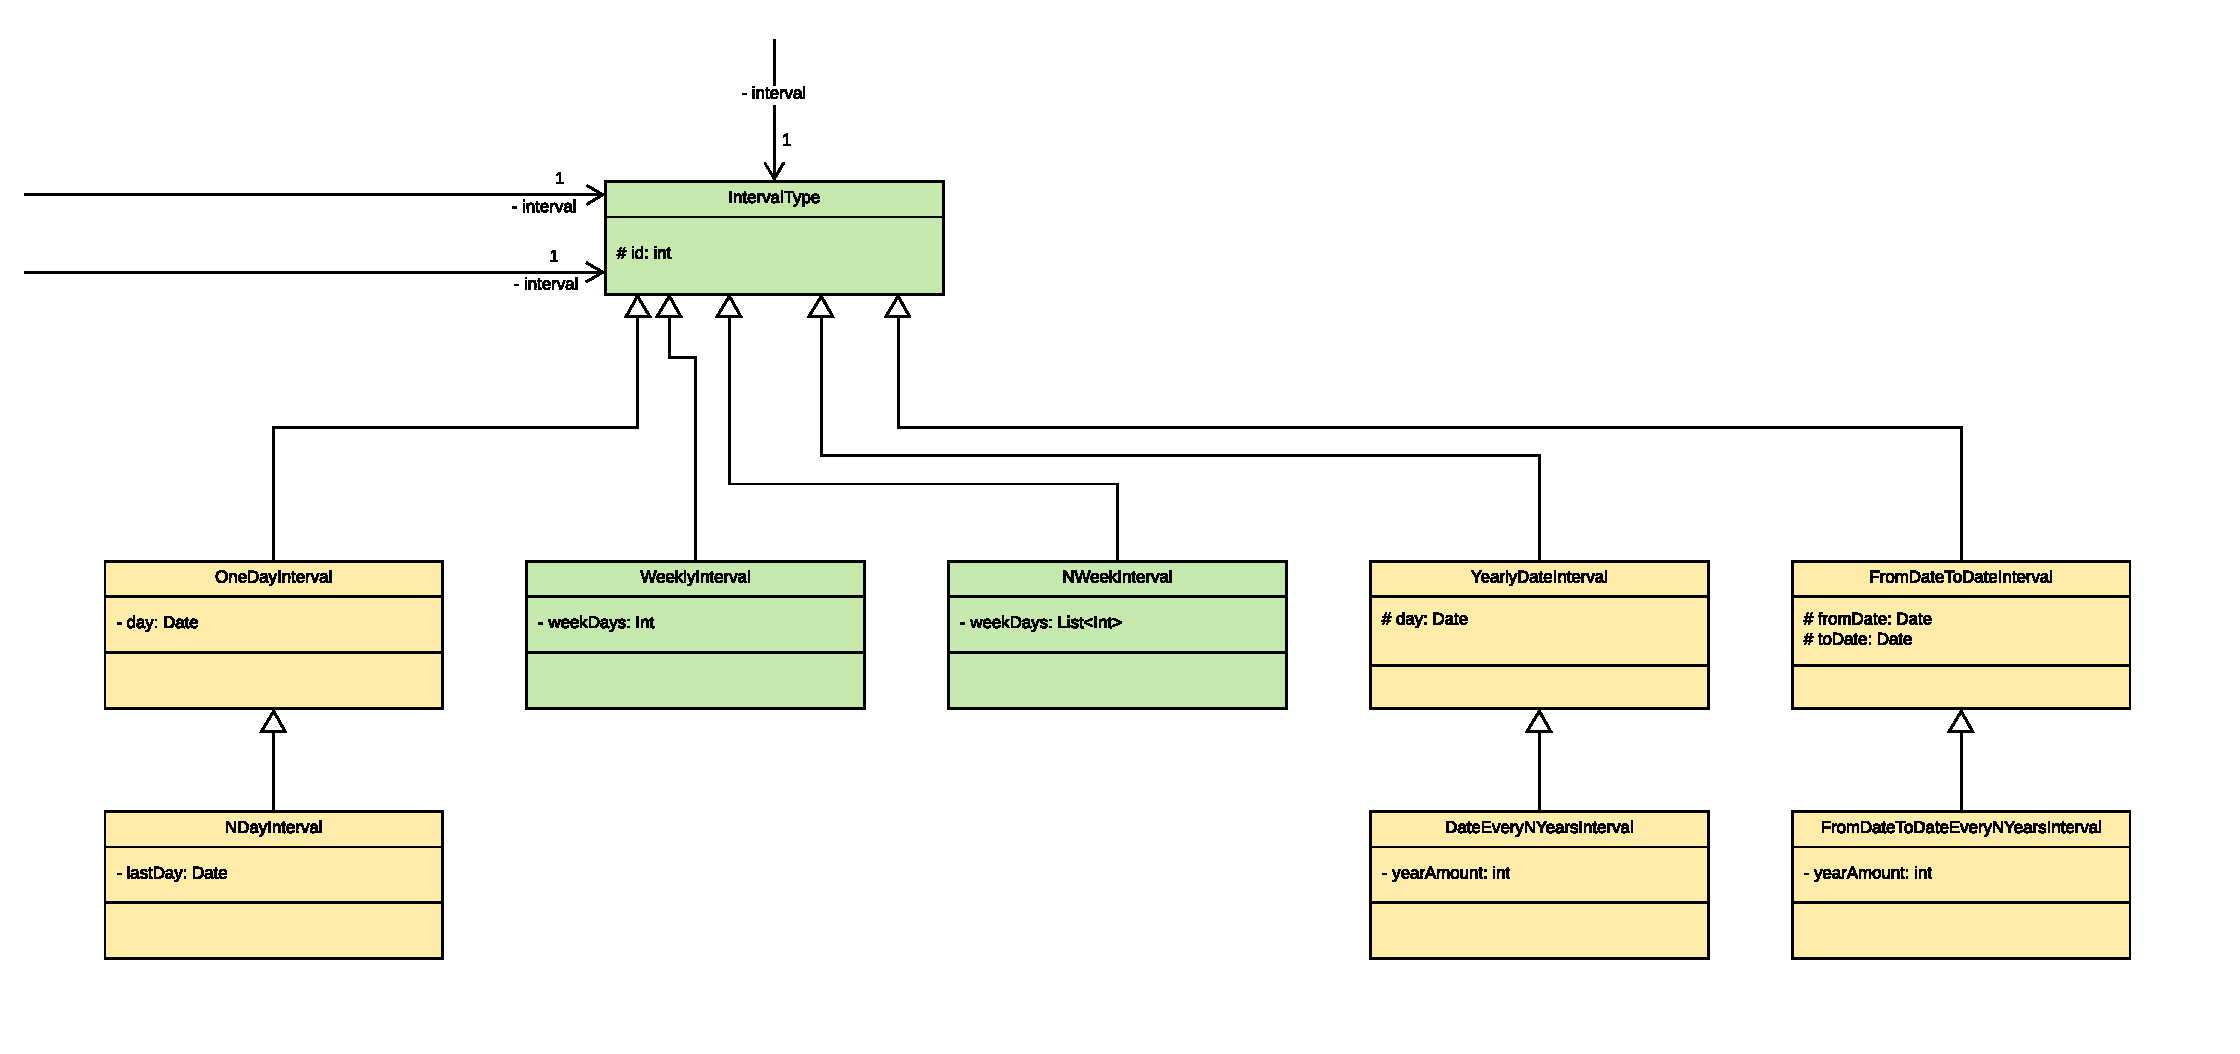
\includegraphics[width=1.0\textwidth]{pdfs/Interval1}
	       % \caption[Předešlý návrh entity \texttt{Interval}]{Návrh entity \textit{Interval} podle doménovém modelu z~předmětu BI-SP2}\label{image:Interval1}
        % \end{figure}
        Prvním takovým požadavkem je změna entity \verb|Interval| (viz obrázek \ref{image:Interval1}), která je v~projektu široce využívaná. Návrh řešení tohoto problému bude popsán v~sekci \ref{navrh:upravy}. Zde bude popsán pouze problém samotný. Entita \verb|Interval| reprezentuje časové rozmezí pro pečovatelské dny, opakované události, nastavení alimentů a navazující požadavky na ně na změny a historické záznamy.
            
        Jádro problému je v~tom, že entita je navržena pomocí generalizace, neboli dědičnosti z~hlediska implementace. Takový návrh dává možnost vytvořit konkrétní typ intervalu pomocí zvolení odpovídající třídy. Na druhou stranu takový návrh působí komplikaci při implementaci a současně nepokrývá všechny možné případy využití intervalů. Například, není možné sestavit interval, který se bude opakovat každý poslední den měsíce. Pokud bychom se chtěli držet aktuální implementace a zároveň pokrýt všechny možné případy, ztratili bychom přehlednost zvolení správné třídy při vytváření instance.
            
        Dalším problémem návrhu entity \verb|Interval| je provázanost s~pečovatelskými dny. Při návrhu frontendové části aplikace bylo zjištěno, že dlouhodobá nastavení pečovatelských dnů rodičů nepotřebují komplikované nastavení a zároveň by potřebovaly mít odkazy na~konkrétního rodiče, který je zodpovědný za dítě v~tento den nebo časový úsek. Proto je potřeba oddělit tyto intervaly pečovatelských dnů zvlášť od ostatních intervalů.
    
    \subsection{Alimenty}
        \begin{figure}\centering
	        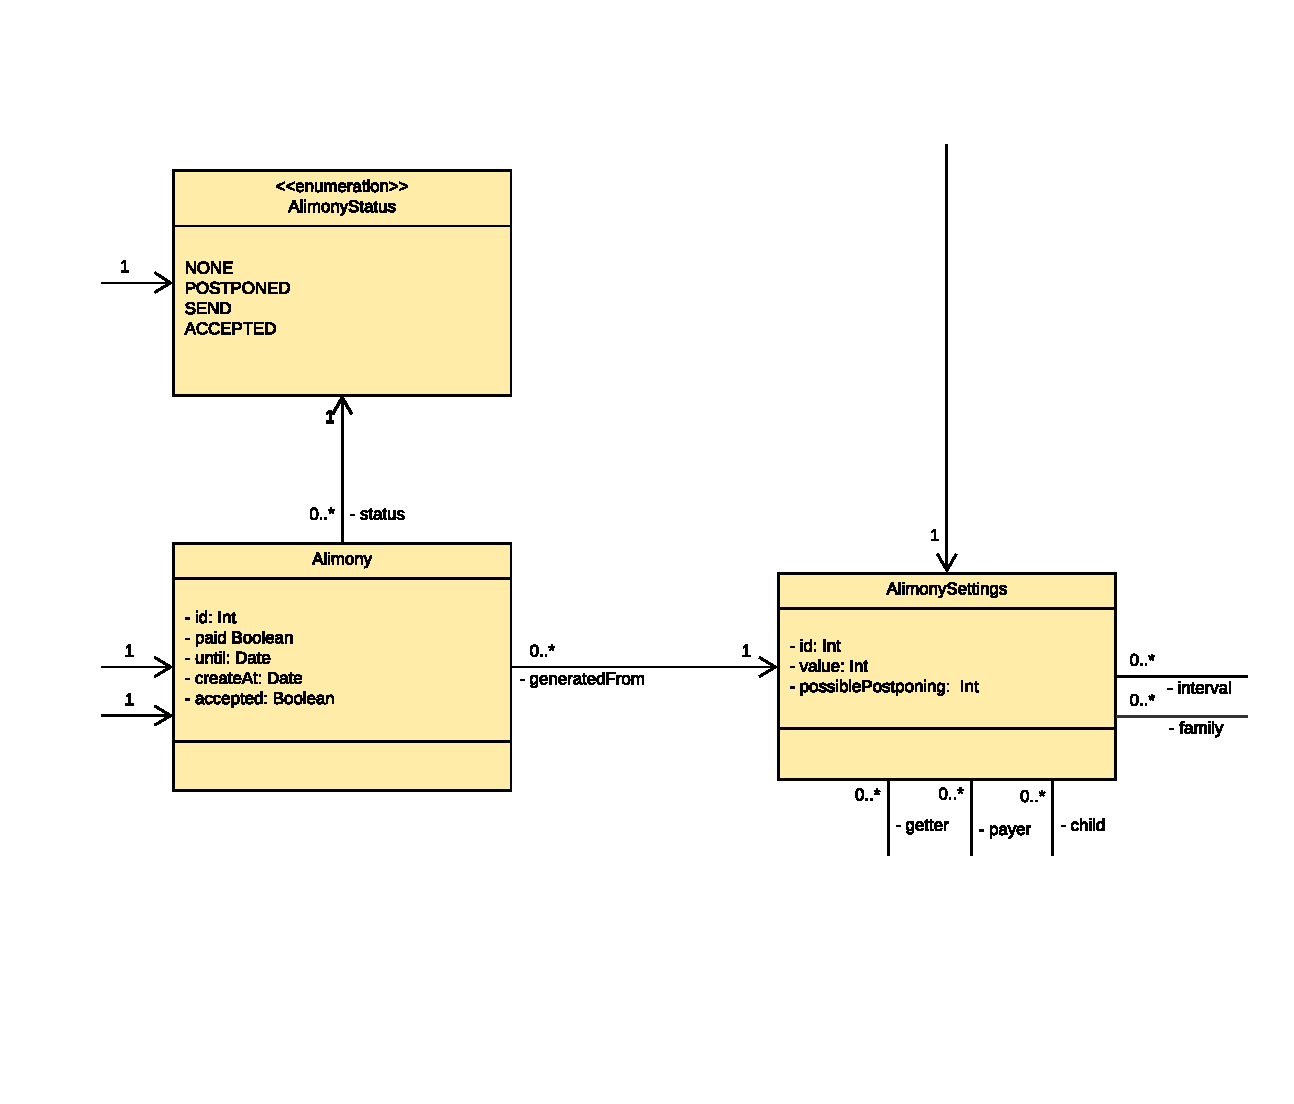
\includegraphics[width=1.0\textwidth]{pdfs/AlimonyDraft1}
	        \caption[Návrh entit \texttt{Alimony} a \texttt{AlimonySettings}]{Návrh entit \texttt{Alimony} a \texttt{AlimonySettings} podle doménového modelu z~předmětu BI-SP2}\label{image:aliomny-draft1}
        \end{figure}
        Entita \verb|Alimony| reprezentuje alimenty, které jeden rodič má posílat druhému rodiči. Jedna instance odpovídá alimentům za jeden měsíc. Předešlý návrh popisuje entitu a její navázanost na entitu \verb|AlimonySettings| (viz obrázek \ref{image:aliomny-draft1}). Nastavení alimentů definují dlouhodobou konfiguraci. Potom se na základě této konfigurace vytváří jednotlivé instance alimentů. Nastavení se definují v~rámci jedné rodiny. V~případě potřeby mají rodiče možnost rozdělit alimenty do několika nastavení, které budou současně validní.
        
        Hlavní problém je v~tom, že instance alimentů by se měly vytvářet nezávisle na frontendové části aplikace, což není popsáno v~předešlém návrhu aplikace. Podrobně návrh řešení problému bude podrobně popsán v~sekci \ref{navrh:upravy:alimenty}.
        
        Dodatečný požadavek frontendového týmu se týká entity \texttt{Alimony} samotné. Za účelem zjednodušení návrhu frontendové části aplikace je potřeba přidat závislost na entitu \texttt{Family}. % V takovém pŕípade aplikace může ihned po nalazení novych alimentu rict uZivateli ktere rodine patri tyto alimenty.
        
    \subsection{Pečovatelské dny}\label{analyza:pozadavky:caredays}
        Než se začneme zabývat podrobným popisem problému, je potřeba popsat účel této entity a její využití backendem a frontendem. Tato entita reprezentuje jednorázový interval nebo opakující se interval pečovatelských dnů jednoho z~rodičů nebo ostatních členů rodiny. Pro rozlišování pečovatelských dnů různých členů rodiny má každý uživatel přiřazenou vlastní barvu. Tato entita se~používá pro dva účely. První a nejdůležitější účel je nastavení pečovatelských dnů pro rodiče. Nastavení musí pokrývat všechny dny kalendáře. Dítě by nemělo mít ve svém kalendáři den, který není označen žádnou barvou a zároveň by neměly vznikat konflikty. Druhým účelem jsou jednorázové změny pečovatelských dnů. Tyto změny jsou vyžadovány pro případy, kdy dlouhodobé nastavení kalendáře neplatí. Příkladem může být výlet dítěte k~prarodičům. Během tohoto časového intervalu nejsou rodiče zodpovědní za dítě, proto je~potřeba uvést jednorázovou změnu do kalendáře, která zaznamená tuto situaci. Jiným příkladem je předání péče jednoho rodiče druhému, což může nastat z~různých důvodu.

        \begin{figure}\centering
            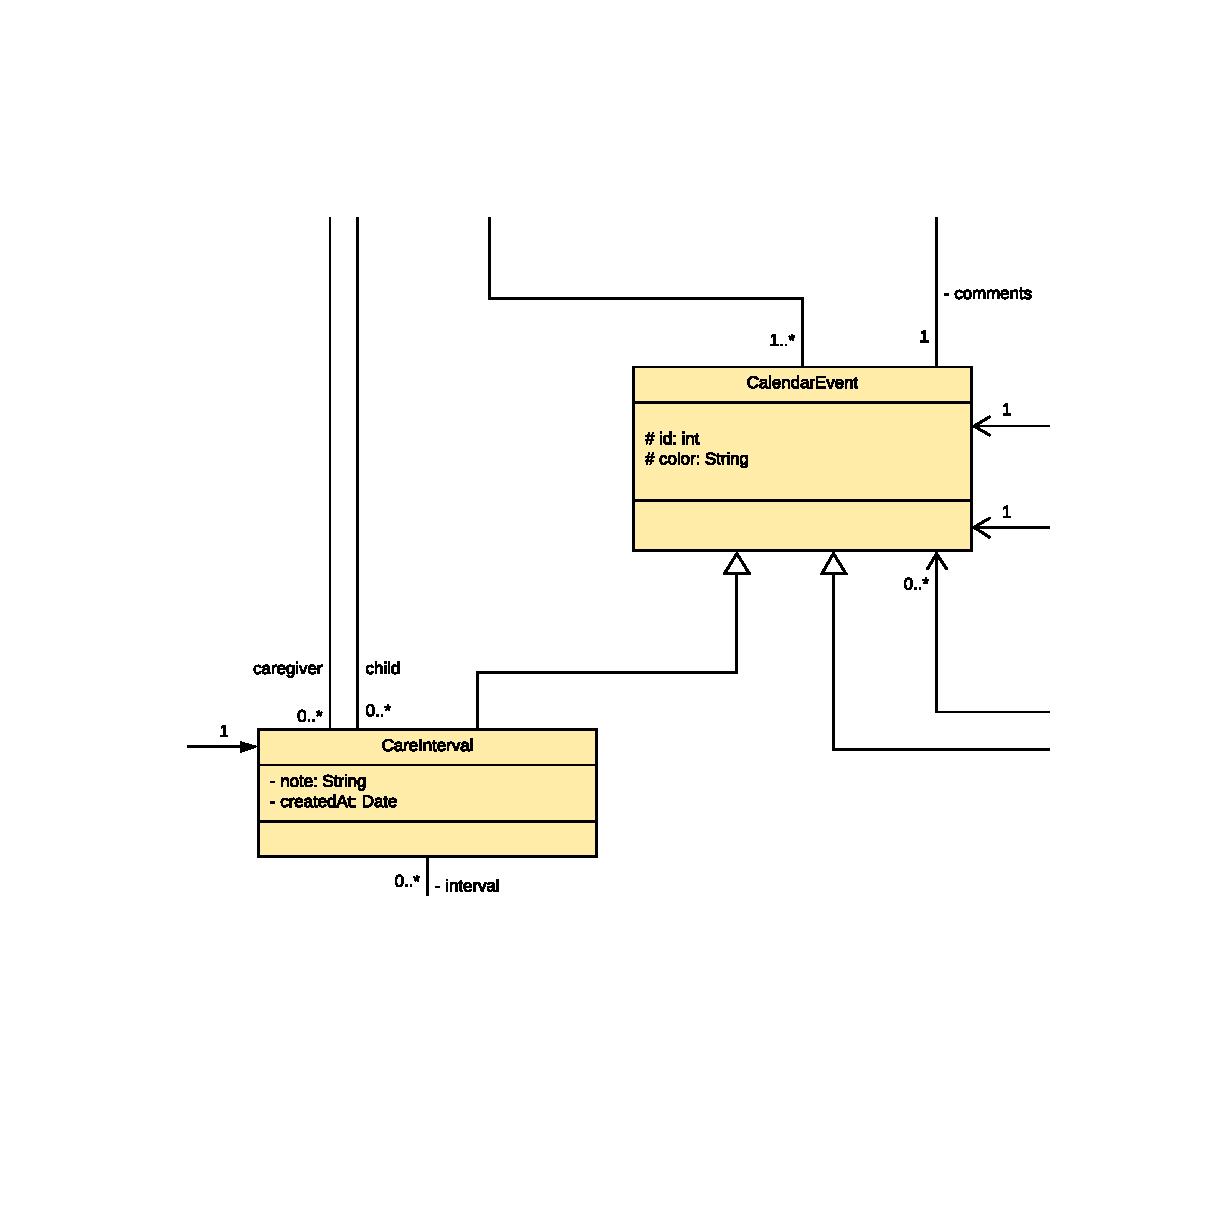
\includegraphics[width=1.0\textwidth]{pdfs/CareDays1}
            \caption[Předešlý návrh pečovatelských dnů]{Návrh pečovatelských dnů podle doménového modelu předmětu BI-SP2}\label{image:caredays1}
        \end{figure}
        Aktuální návrh pečovatelských dnů je navržen příliš komplikovaně (viz obrázek \ref{image:caredays1}) a současně zahrnuje dva různé případy využití: jednorázové změny pečovatelských dnů členů rodiny a dlouhodobá nastavení pečovatelských dnů rodičů. Dlouhodobá nastavení pečovatelských dnů rodičů nevyžadují komplikovaný návrh intervalů (viz sekci \ref{analyza:pozadavky-frontendu}), proto je potřeba oddělit řešení tohoto problému. Také je potřeba přidat odkaz na konkrétního rodiče, který je zodpovědný za tento den pro zjednodušení práce s~touto entitou v~rámci frontedové části aplikace. Jednorázové změny pečovatelských dnů je druhý problém, který je potřeba oddělit. Návrh této entity je podobnější aktuálnímu návrhu, protože tyto změny mohou vyžadovat složitá pravidla opakování. Navržené změny a následné implementace budou popsány v~sekci \ref{navrh:upravy:caredays}.
        
     \subsection{Oznámení}
        % \begin{figure}\centering
        %     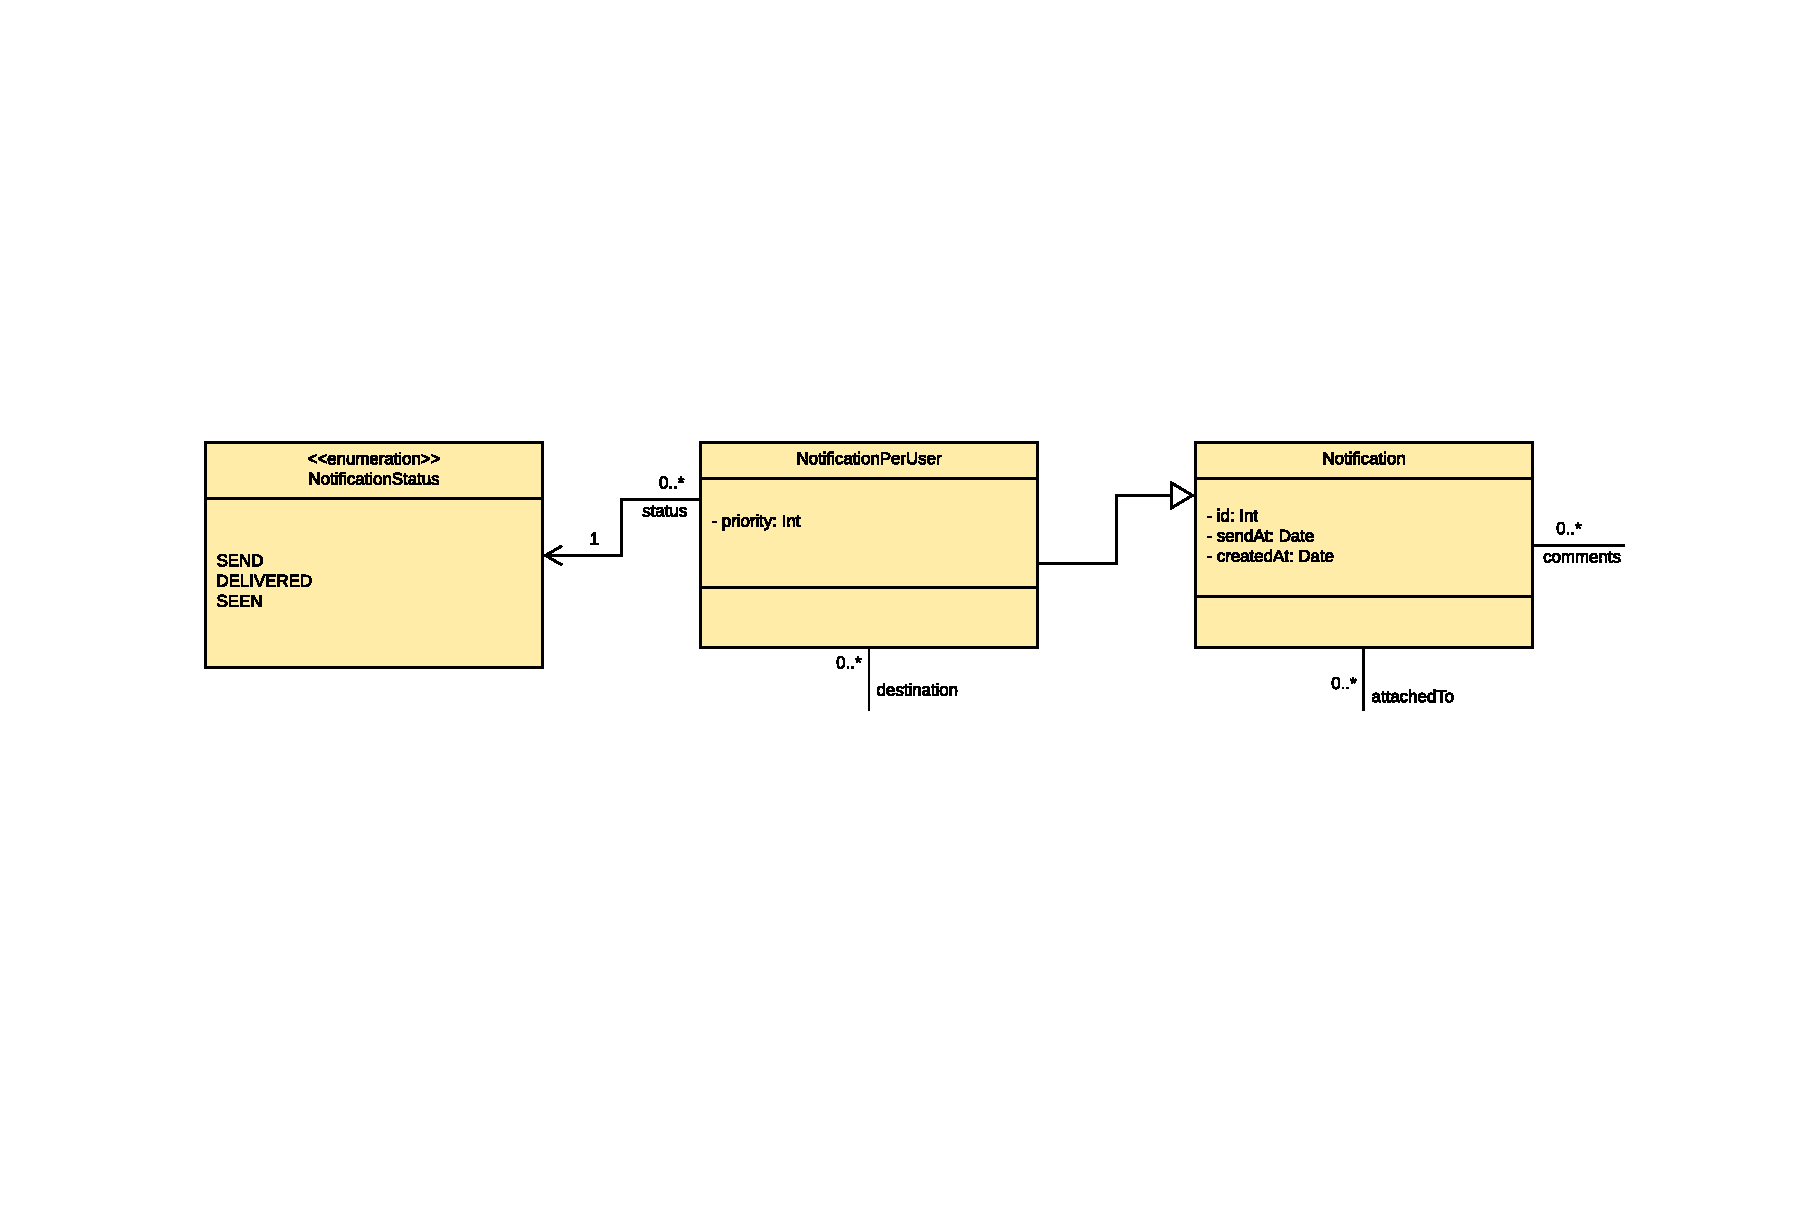
\includegraphics[width=1.0\textwidth]{pdfs/Notification1}
        %     \caption[Předchozí návrh oznámení]{Návrh oznámení podle doménového modelu předmětu BI-SP2}\label{image:notification1}
        % \end{figure}
        Dosavadní návrh oznámení reprezentuje upozornění uživatele o~požadavku na~změnu (viz obrázek \ref{image:notification1}). Po provedení částečné implementace frontendové a backendové částí bylo zjištěno, že návrh oznámení potřebuje úprav ve~dvou různých směrech. Prvním směrem je zavedení různých typu oznámení, například oznámení pomocí e-mailu nebo SMS zprávy. Současná implementace frontendové části aplikace vyžaduje zavedení typu upozornění, které by reprezentovaly upozornění v~rámci Android aplikace. 
        Tyto upozornění vyžadují specifické nastavení entity, například možnost přečtení jednotlivé instance. Druhým směrem je rozšíření seznamu událostí, které mohou působit vzniku oznámení. Příčinami mohou být:
        \begin{itemize}
            \item změny pečovatelských dnů;
            \item alimenty;
            \item změny nastavení alimentů;
            \item potřeby dítěte;
            \item změny v~rámci rodiny.
        \end{itemize}
        Podle požadavků frontendové části aplikace je také potřeba uvádět příčinu vniku upozornění v~každé instanci. Příčinou může být jedná z~výše zmíněných událostí. Za účelem navržení kvalitnějšího API je také potřeba přidat možnost přečíst najednou všechna upozornění, která uživatel má. Kompletní řešení problému bude popsáno v~sekci \ref{navrh:upravy:notification}.
        % Také frontendová část aplikace vyžaduje přizpůsobení oznámení upozorněním v rámci Android aplikace, což vyžaduje úpravu atributů. Také je potřeba specifikovat která událost způsobilá vytvoření tohoto oznámení a přidat typ této události podle výše uvedeného seznamu. Za účelem navrženi kvalitnějšího API je také potřeba přidat možnost přečíst všechny upozornění, které má uživatel, najednou. Řešení problému bude popsáno v sekci \ref{navrh:upravy:notification}.
        
            
            % reprezentuje libovolný typ oznámení. Tudíž oznámení pomocí elektronické pošty a pomocí upozornění v telefonu jsou reprezentovány pomocí stejné entity.
            
            % Frontedová část aplikace vyžaduje přizpůsobení oznámení upozorněním v rámci Android aplikace, což je konkretním typem oznámení a vyžadují sadu specifických atributu:
            % \begin{itemize}
            %     \item ID
            %     \item 
            % \end{itemize}
            % Řešení tohoto problému bude popsáno v sekci \ref{navrh:upravy:notification}
            
    % \section{Analýza konkurence}
    %     Tento návrh...
% \section{Analýza testování}

\section{Analýza bezpečnosti}
    V~této sekci budou popsány procesy, které by měly zaručovat bezpečnost aplikace ze strany serverového backendu.
    
    \subsection{Role}\label{analyza:bezpecnost:role}
    
    % Aplikace je navržená tak, že první věc, kterou uživatel udělat, je registrace. Uživatel potřebuje zvolit jméno, příjmení, email a heslo. Na základě těchto údajů se vytváří účet uživatele. V Doménovém modelu tato třída se jmenuje \texttt{User}. V tento okamžik uživatel má role \texttt{USER}, která mu nadává možnost udělat jenom omezený počet věcí.  
        % \begin{figure}\centering
	       % 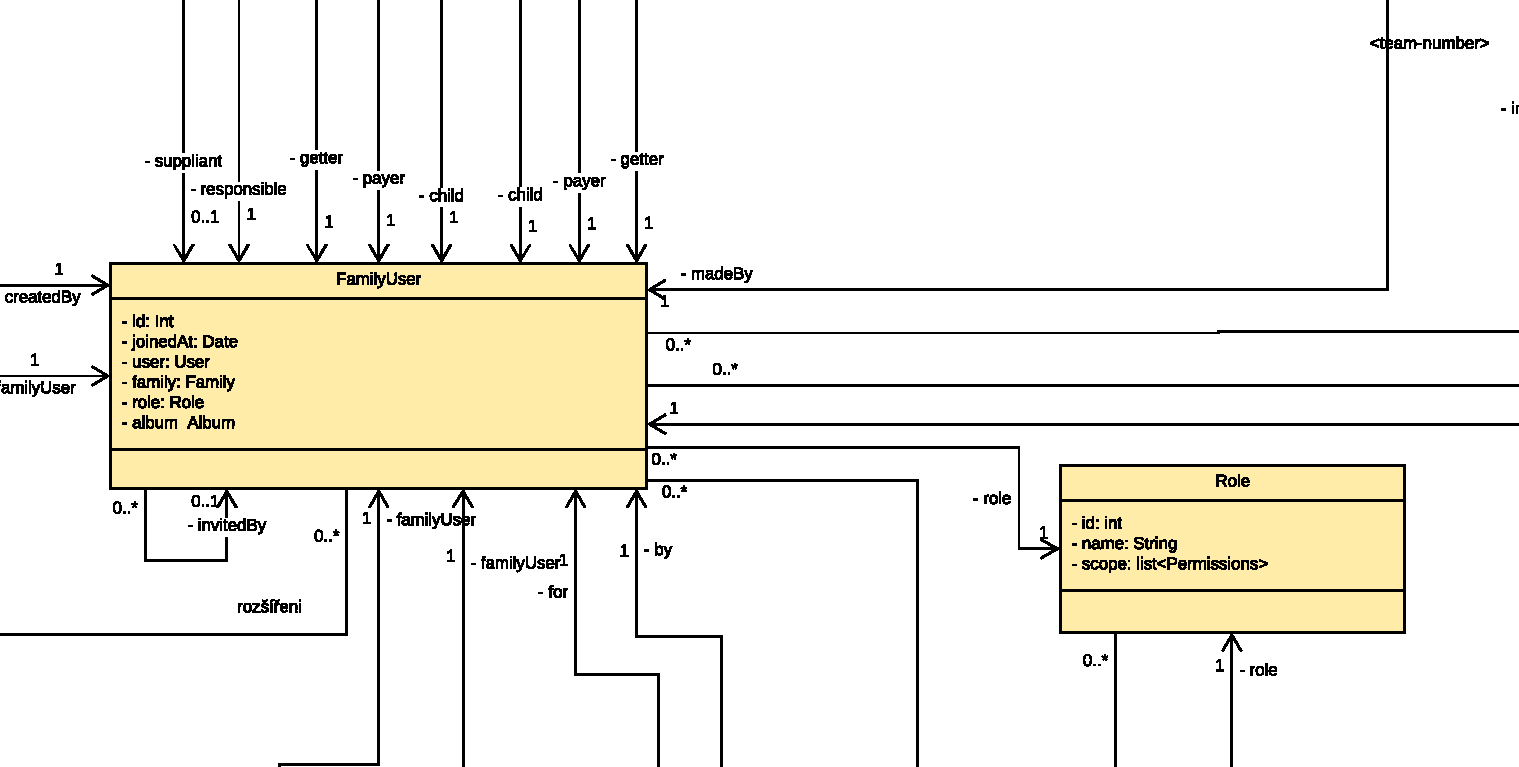
\includegraphics[width=1.0\textwidth]{pdfs/Role1}
	       % \caption[Návrh \texttt{Role}]{Návrh entity \texttt{Role} podle doménového modelu z~předmětu BI-SP2}\label{image:Role1}
        % \end{figure}
        Než se uživatel přihlásí do rodiny, nemá žádnou roli. Po přihlášení do rodiny má uživatel roli v~rámci přihlášené rodiny (viz obrázek \ref{image:Role1}), podle které se~mohou lišit jeho přístupová práva. Hlavní rolí v~aplikaci je rodič. Uživatel s~takovou rolí má přístup ke všem potřebám dítěte a všem záznamům v~kalendáři. Rodič také může vytvářet pozvání do rodiny pro libovolného uživatele a nastavit mu libovolnou roli, včetně role rodiče. Mimořádnou rolí v~rámci systému je dítěte. 
        Uživatel s~takovou rolí nemůže vlastnit pečovatelský den nebo splnit přání. Přihlášení dítěte muže proběhnout i bez vytvoření klasického uživatele v~rámci systému. Ostatní uživatelé v~rodině mají roli příbuzných. 
    
    \subsection{Autorizace}
        Návrh bezpečné aplikace nebyl cílem předmětů zmíněných v~sekcích \ref{analyza:navrh:sp1} a \ref{analyza:navrh:sp2}. Proto návrh a předešla implementace neobsahuje proces přihlašování uživatele do systému. Navržené procesy autentizace a autorizace budou podrobně popsány v~sekci \ref{navrh:bezpecnost}.
        
\section{Analýza testování}\label{analyza:testovani}
    Dosavadní návrh neobsahuje informaci o~implementaci testování. Ale předešlá implementace obsahuje pouze jeden test, který se zaměřuje na ověření, jestli se načetl {kontext aplikace}\footnote{Pokročilý kontejner, který funguje podobně jako \texttt{BeanFactory}. Načítá definice beanů, provazuje je a vydává v~případě nutnosti.} (viz obrázek \ref{code:test-context-loads1}). Cela implementace testování aplikace bude provedená v rámci této bakalářské práce.
    \begin{figure}
    \begin{minted}[frame=lines,
        framesep=2mm,
        baselinestretch=1.2,
        fontsize=\footnotesize,
        linenos]{java}
@RunWith(SpringRunner::class)
@SpringBootTest
class RozvodyApplicationTests {

    @Test
    fun contextLoads() {
    }

}
        \end{minted}
        \caption{Ukázka předešlého testování} 
        \label{code:test-context-loads1}
        \end{figure}
        
\section{Průběžná integrace}\label{analyza:ci}
    Na začátku je potřeba popsat pravidla zavedená pro distribuovaný systém správy verzí -- Git -- před začátkem implementace serveru. Proces vývoje byl rozdělen do dvou hlavních větví. První větev reprezentuje aktuální verzi aplikace a je označena jako \enquote{master}, což je implicitní větev v~rámci Git. Druhá větev je označena jako \enquote{dev} a je určena pro proces vývoje. Pro implementaci jednotlivých úkolů je potřeba udělat kopii této větvi a po vyřešení úkolu je potřeba zařadit všechny změny zpět do větve \verb|dev|. Takový přístup dává možnost pracovat na stejném projektu několika programátorům najednou a s~jistotou uschovávat vlastní změny na server bez ohledu na jejich kompletnost.
    
    Vedoucím této bakalářské práce a současně vedoucím tohoto projektu byl poskytnut server pro testování, dostupný z~IP: \enquote{http://37.46.80.230/}. Větve \verb|master| a \verb|dev| se automaticky nasazují po aktualizaci. Aplikace uložena do~větve \verb|master| je dostupná na portu 8998. Aplikace uložena do větve \verb|dev| je dostupná na portu 8778.